\section{Differentiable Automata}
\label{sec:differentiable_automata}

Modern deep learning relies on the fact that core functions are differentiable
(or sub-differentiable). This is important to any type of gradient-based
numerical optimization, of which the most commonly used are variations of
stochastic gradient descent. The parameters, $\theta$, of the model are
specified in tensors. The objective function, $f(\theta, \vx, \vy)$, is a
function of the parameters and the input data $\vx$ and $\vy$. The parameters
can then be optimized to improve the objective with variations of a simple
update rule:

$$
\theta_t = \theta_{t-1} + \alpha \, \nabla_{\theta} f(\theta_t, \vx, \vy),
$$

where $\alpha$ is the learning rate, and $\nabla_{\theta}$ is the gradient
operator which we describe in more detail below. This update applies equally
well to parameters in graphs as it does to tensors. The main challenge is
computing gradients, the subject of this section.


\subsection{Derivatives}

Many operations used with vectors, matrices, and $n$-dimensional tensors are
differentiable. This means we can compute the change in any of the output
elements with respect to an infinitesimal change in any of the input elements.
For example, consider a vector $\vz = f(\vx, \vy)$ which is the output of a
function of two vectors $\vx$ and $\vy$. The Jacobian of $\vz$ with respect to
$\vx$ is the  natrix of partial derivatives with entries $\frac{\partial
\vz_i}{\partial \vx_j}$. The gradient is defined as the tensor of partial
derivatives of a scalar function. So if $f(\vx) \in \mathbb{R}$ is a scalar
function, then the gradient is:

$$
\nabla f(\vx) = \left[ \frac{\partial f(\vx)}{\partial \vx_{1}}, \ldots,
    \frac{\partial f(\vx)}{\partial \vx_{n}}  \right]^\top.
$$

In the same way, we can compute partial derivatives of the arc weights of an
output graph for a given operation with respect to the arc weights of any of
the input graphs. Take the concatenation operation as an example. Suppose we
are given two graphs, $\gA$ and $\gB$, and we construct the concatenated graph
$\gC = \gA \gB$ as in figure~\ref{fig:concat_grad}.

\begin{figure}
    \centering
    \begin{subfigure}[b]{0.23\textwidth}
        \centering
        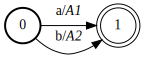
\includegraphics[scale=0.6]{figures/concat_grad_A}
    \end{subfigure}
    \begin{subfigure}[b]{0.23\textwidth}
        \centering
        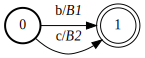
\includegraphics[scale=0.6]{figures/concat_grad_B}
    \end{subfigure}
    \begin{subfigure}[b]{.52\textwidth}
        \centering
        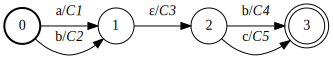
\includegraphics[scale=0.6]{figures/concat_grad_C}
    \end{subfigure}
    \caption{The concatenation of the graphs $\gA$ (left) and $\gB$ (middle)
    produces $\gC$ (right). For each graph the arc weights are shown as
    variables on the edges.}
    \label{fig:concat_grad}
\end{figure}

For each of the arc weights $C_i$ in the concatenated graph $\gC$, we can
compute the partial derivative with respect to the arc weights of $\gA$ and
$\gB$. For any arc in $\gC$, it either has a corresponding arc in $\gA$ or
$\gB$ from which it gets its weight, or it has a weight of zero. The partial
derivative of an output arc weight $C_i$ with respect to an input arc weight
$A_j$ or $B_j$ is $1$ if the two arcs correspond and $0$ otherwise. For
example, in the graphs in figure~\ref{fig:concat_grad} we have:

$$
\frac{\partial C_1}{\partial A_1} = 1,
    \quad \frac{\partial C_2}{\partial A_2} = 1,
    \quad \frac{\partial C_4}{\partial B_1} = 1,
    \quad\textrm{and}\quad \frac{\partial C_5}{\partial B_2} = 1.
$$

The remaining partial derivatives are all $0$. For example, for $C_1$ we have:

$$
\frac{\partial C_1}{\partial A_2} = 0,
    \quad \frac{\partial C_1}{\partial B_1} = 0,
    \quad \textrm{and} \quad \frac{\partial C_1}{\partial B_2} = 0.
$$

In the following, I use the notation $\frac{\partial \gC}{\partial \gA}$ to
generalize the Jacobian to graphs. This Jacobian is a data structure which
contains the partial derivatives $\frac{\partial C_i}{\partial A_j}$ for all
arc weights $C_i$ in $\gC$ and $A_j$ in $\gA$. Another way to view this
Jacobian is as a set of graphs $\frac{\partial C_i}{\partial \gA}$ indexed by
$i$ which are the same size as $\gA$. Alternatively we can view the Jacobian as
a set of graphs $\frac{\partial \gC}{\partial A_j}$ indexed by $j$ which are
the same size as $\gC$. This is analogous to viewing the Jacobian of a
vector-valued function either as a set of columns or a set of rows.

\begin{example}
Compute the partial derivatives of the arc weights of the closure of the graph
$\gA$ from figure~\ref{fig:concat_grad} with respect to the input arc
weights. The closure, $\gA^*$, is in figure~\ref{fig:closure_grad}.
\end{example}

\begin{proof}[\unskip\nopunct]

\begin{figure}
    \centering
    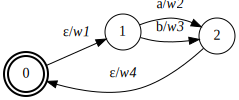
\includegraphics[scale=\dotscale]{figures/closure_grad}
    \caption{The closure of the graph $\gA$ from figure~\ref{fig:concat_grad}.
    The weights are denoted by the variables $w_i$.}
    \label{fig:closure_grad}
\end{figure}

The non-zero partial derivatives are:

$$
\frac{\partial w_2}{\partial A_1} = 1
    \quad \textrm{and} \quad \frac{\partial w_3}{\partial A_2} = 1.
$$

The remaining partial derivatives are zero:

$$
\frac{\partial w_1}{\partial A_1} = 0, \quad \frac{\partial w_1}{\partial A_2} = 0,
    \quad \frac{\partial w_2}{\partial A_2} = 0,
    \quad \frac{\partial w_3}{\partial A_1} = 0,
    \quad \frac{\partial w_4}{\partial A_1} = 0,
    \quad \textrm{and} \quad \frac{\partial w_4}{\partial A_2} = 0.
$$
\end{proof}

\begin{example}
Compute the partial derivatives of the intersected automata weights $w_i$ with
respect to the input arc weights $A_j$ for graph $\gA$ and $B_k$ for graph
$\gB$ shown in figure~\ref{fig:intersect_grad_inputs}.
\end{example}

\begin{figure}
    \centering
    \begin{subfigure}[b]{0.3\textwidth}
        \centering
        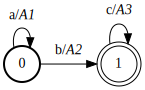
\includegraphics[scale=\dotscale]{figures/intersect_grad_1}
    \end{subfigure}
    \begin{subfigure}[b]{0.68\textwidth}
        \centering
        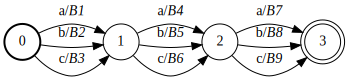
\includegraphics[scale=\dotscale]{figures/intersect_grad_2}
    \end{subfigure}
    \caption{We would like to compute the derivative of the intersected graph's
    arc weights with respect to the arc weights in the two input acceptors
    $\gA$ and $\gB$. The arc weights are labeled with the variable names $A_j$
    and $B_k$.}
    \label{fig:intersect_grad_inputs}
\end{figure}

\begin{figure}
    \centering
    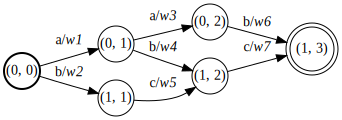
\includegraphics[scale=\dotscale]{figures/intersect_grad}
    \caption{The intersected graph of the two acceptors $\gA$ and $\gB$ in
    figure~\ref{fig:intersect_grad_inputs}.  The weights are denoted as
    variables $w_i$ on the edges.}
    \label{fig:intersect_grad}
\end{figure}

\begin{proof}[\unskip\nopunct]
The partial derivative $\frac{\partial w_i}{\partial A_j}$ is $1$ if the weight
$w_i$ came from $A_j$ and zero otherwise. The derivatives with a value of $1$
for graph $\gA$ are:

$$
\frac{\partial w_1}{\partial A_1}, \; \frac{\partial w_2}{\partial A_2}, \;
    \frac{\partial w_3}{\partial A_1}, \; \frac{\partial w_4}{\partial A_2}, \;
    \frac{\partial w_5}{\partial A_3}, \; \frac{\partial w_6}{\partial A_2}, \;
    \textrm{and} \;\; \frac{\partial w_7}{\partial A_3}.
$$

The derivatives with a value of $1$ for graph $\gB$ are:

$$
\frac{\partial w_1}{\partial B_1}, \; \frac{\partial w_2}{\partial B_1}, \;
    \frac{\partial w_3}{\partial B_4}, \; \frac{\partial w_4}{\partial B_5}, \;
    \frac{\partial w_5}{\partial B_6}, \; \frac{\partial w_6}{\partial B_8}, \;
    \textrm{and} \;\; \frac{\partial w_7}{\partial B_9}.
$$

The remaining derivatives for both graphs are zero.
\end{proof}

\subsection{Automatic Differentiation}

In the previous section we saw how to compute derivatives for some common
automata operations. Automatic differentiation greatly simplifies the process
of computing derivatives for arbitrary compositions of operations. In this
section, we will discuss \emph{reverse-mode} automatic differentiation at a
high-level.

Reverse-mode automatic differentiation proceeds in two steps. First, a forward
pass computes all of the operations. Then, a backward pass computes the
gradients. During the forward pass the composition of operations is stored in a
computation graph (not to be confused with an automata). Data and metadata are
also cached during the forward pass to make the gradient comptuation more
efficient. There is often a trade-off between memory and compute in that we can
save more intermediate data to reduce the computation required during but
increase the memory required during the bakcward pass.

Consider the graph equation:

\begin{equation}
    \label{eq:compute_graph}
    \LSE\left[ \left(\left(\gA_1 + \gA_2\right) \circ \gX^*\right) \right].
\end{equation}

This equation can be represented in the computation graph in
figure~\ref{fig:compute_graph}.

\begin{figure}
    \centering
    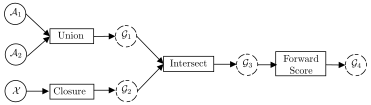
\includegraphics[scale=0.9]{figures/compute_graph}
    \caption{An example of a compute graph for equation~\ref{eq:compute_graph}.
    The solid circular nodes are leaves. The graphs $\gA_1$ and $\gA_2$ are
    parameters, and $\gX$ is input data. The rectangular nodes are operations.
    The dashed circular nodes are graphs computed as the result of an
    operation.}
    \label{fig:compute_graph}
\end{figure}

The leaves of the computation graph (the solid circular nodes with no incoming
arrows) are either parameter graphs or input data graphs. In this case, let's
assume $\gA_1$ and $\gA_2$ are the parameter graphs, and $\gX$ is the graph of
input data. The square nodes are operations, and they are always followed by
output graphs, which are dashed circular nodes.

During the backward pass, the gradients are computed from the output ($\gG_4$
in figure~\ref{fig:compute_graph}) following the arrows in the computation
graph backwards. A graph can only compute its gradient once all of the graphs
downstream of it have had their gradients computed. Thus the backward pass must
be done as a reverse topological traversal of the computation graph.

For example, assume the gradient of the output $\gG_4$ with respect to graph
$\gG_1$ has been computed. This gradient $\frac{\partial \gG_4}{\partial
\gG_1}$ is then used to compute $\frac{\partial \gG_4}{\partial \gA_1}$ and
$\frac{\partial \gG_4}{\partial \gA_2}$. Assuming we know how to differentiate
$\gG_1$ with respect to $\gA_1$ and $\gA_2$, then we can compute the desired
gradients essentially using the chain rule. Assume $g_i$ are the arc weights of
$\gG_1$ and $a_j$ are the arc weights of $\gA_1$, then the chain rule gives:

$$
\frac{\partial \gG_4}{\partial a_j} =
    \sum_{i} \frac{\partial \gG_4}{\partial g_i} \frac{\partial g_i}{\partial a_j}.
$$

This is done recursively at every node in the computation graph until the
gradients for all the leaf graphs are available.

At a high-level any implementation of reverse-mode automatic differentiation is
the same. However, implementations often differ in the details. One simple
approach is to have every output graph record the input graphs from which it
was generated as well as a gradient computation function. The input graphs and
gradient computation function (and any other metadata) can be set during the
forward pass by the operation itself.

For example, after the execution of union, the data structure which holds the
output graph $\gG_1$ could also hold pointers to the inputs $\gA_1$ and $\gA_2$
and a pointer to the gradient computation function for union. A simplified
example of what this data structure might look like is shown in
figure~\ref{fig:grad_data}.

\begin{figure}
    \centering
    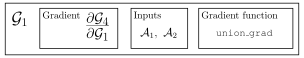
\includegraphics[scale=0.9]{figures/grad_data}
    \caption{The data structure which holds the graph $\gG_1$ as well as the
    data needed to compute the gradient of its inputs. In this case $\gG_1$ was
    the output of a union of $\gA_1$ and $\gA_2$.}
    \label{fig:grad_data}
\end{figure}

Once the gradient for $\gG_1$ is available, the union's gradient function is
called with the inputs $\gA_1$, $\gA_2$, and $\frac{\partial \gG_4}{\partial
\gG_1}$. For $\gA_1$, the union gradient function will compute $\frac{\partial
\gG_1}{\partial \gA_1}$ and use the chain rule as described above to assemble
the desired gradient $\frac{\partial \gG_4}{\partial \gA_1}$. It will do the
same for $\gA_2$.
